\begin{center}
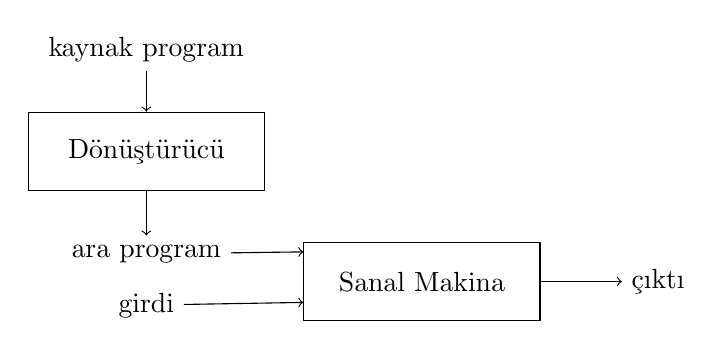
\begin{tikzpicture}[->]

\tikzstyle{rect} = [rectangle, minimum width=3cm, minimum height=1cm,text centered, draw=black]

\node (src_p)   {kaynak program};
\node (translator) [rect, below of=src_p, yshift=-0.3cm] {Dönüştürücü};   
\node (intermediate_p) [below of=translator, yshift=-0.3cm] {ara program};
\node (in) [below of=intermediate_p, yshift=0.35cm] {girdi};
\node (vm) [rect, right of=in, xshift=2.5cm, yshift=0.3cm, ] {Sanal Makina};   
\node (out) [right of=vm,xshift=2cm] {çıktı};

\draw [black](src_p) -- (translator);  
\draw [black](translator) -- (intermediate_p);  
\draw [black](intermediate_p) -- (vm.166);  
\draw [black](in) -- (vm.190);  
\draw [black](vm) -- (out);  

\end{tikzpicture}

Şekil 1.4: Bir hibrid derleyici
\end{center}